\documentclass[hidelinks,a4paper]{article}
    
\usepackage[utf8]{inputenc}
\usepackage[total={15cm,25cm}, top=2cm, left=3cm, includefoot]{geometry}
\usepackage{amsmath,amsfonts,amssymb}
\usepackage{graphicx}
\usepackage{hyperref}
\usepackage{fancyhdr}
\usepackage{caption}
\usepackage{subcaption}
\usepackage{biblatex}

\addbibresource{Report.bib}
    
\author{Jakub Šťastný}
\title{Substituting GPS with Gyroscope and Accelerometer}
\date{\today}
\makeatletter

\pagestyle{fancy}
\fancyhf{}
\rhead{\@author}
\lhead{\@title}
\lfoot{\thepage}
\rfoot{\today}


\begin{document}
% TITLE PAGE
\pagenumbering{gobble}
\begin{titlepage}
    \thispagestyle{plain}
    \begin{center}
        \Large
        \textbf{\@title}
            
        \vspace{0.4cm}
        \large
            
        \vspace{0.8cm}
        \textbf{\@author} \\
        {\small Student number: 03729788}\\
        {\small Course: Real-time Systems [IN2060] }
        
        \vspace{16cm}
        \textbf{Abstract}
    \end{center}
    % ABSTRACT
    I have built a device that measures the user's current position and speed mainly using GPS and that tries to substitute the GPS with a gyroscope and an accelerometer in case of losing the GPS signal. I will describe the hardware from which the device is built in the first part. In the second part I will talk about the processing of accelerometer data, reducing measurements errors and calculating the final position of the device in the earth coordinates system. In the last part I will talk about the precision of the device and about the cause of the errors. 
\end{titlepage}
\makeatother

% SECTION 0: PROJECT DESCRIPTION
\pagenumbering{arabic}
\section{Project description}
In this project I have built the device that shows the user his/her current position and speed on the display in a real time. In a normal case, the device is using only a GPS chip in order to get the information about the current location. But there are many cases when we lose a GPS signal. For example inside some buildings, between high mountains, in tunnels, etc. We want to have the device still running in these cases, so we have to substitute the GPS with some other alternative that is independent of the quality of a signal. I decided for the gyroscope and accelerometer that can measure our acceleration and angular speed, which can be using double integration converted to the relative location\footnote{The location difference between our current location and location before the start of the acceleration measurement} and combined with the last location that the GPS measured before it lost the signal, in order to calculate the current location. With this technique we can keep the device running and providing the output to the user for the whole time even if we do not have any signal.\par
Besides the controller board, accelerometer, gyroscope and display, the device contains two additional buttons. One of them is used for the (re)calibration of the device (described later). The second button is present only for the testing purpose and is used for the simulation of the situation that we do not have any GPS signal. If a user presses this button, he/she turns on the testing mode so that the device does not use any information from the GPS, even if it has a GPS signal and calculates the current speed and location only using the accelerometer and gyroscope data in order to simulate and test the situation that we do not have a GPS signal. If the user presses the button again, the testing mode is turned off and the device is working normally.\par
The device also has one additional LED, which indicates that the testing mode is turned on.\\\par
The whole project including all source codes, this report and photos is available on my github.\\
\url{https://github.com/StastnyJ/accelerometerPositionReader}

% SECTION 1: HARDWARE
\section{Used hardware}
For this project I used following hardware:

\begin{enumerate}
    \item LILYGO TTGO T-Beam V1.1\footnote{Detailed description: \url{https://www.banggood.com/LILYGO-TTGO-T-Beam-ESP32-433-or-868-or-915-or-923Mhz-V1_1-WiFi-Wireless-bluetooth-Module-GPS-NEO-6M-SMA-LORA32-18650-Battery-Holder-With-OLED-p-1545070.html}}
    \item MPU-6050 3 Axis Gyro With Accelerometer\footnote{Detailed description: \url{https://www.banggood.com/3pcs-6DOF-MPU-6050-3-Axis-Gyro-With-Accelerometer-Sensor-Controller-Module-p-1430733.html}}
    \item OLED 128x64 I2C SSD1315 12864 LCD Screen Display module\footnote{Detailed description: \url{https://www.amazon.com/Serial-Display-Module-SSD1315-arduino/dp/B07Y5HNJGL}}
    \item 2 Buttons, 1 LED and 18650 Battery
\end{enumerate}

\subsection{Controller board}

As a microcontroller for this project, I used LILYGO TTGO T-Beam board version 1.1. This board is based on the ESP32 processor. It offers 4 MB Flash memory and 4 MB of PSRAM. The board also contains 2 additional modules. First of them is module LoRa32 which is used for wide area communication via bluetooth and WiFi. I haven't used this module for the project. The second and for the project more important module is the NEO-6M module used for GPS. This module can measure current gps location with the accuracy up to 2.5 meters\footnote{This accuracy can be achieved only with a quite good antenna or a clear sky view. With the antenna I used for the project is the accuracy between 15 and 20 meters.}. This module communicates with the ESP processor via integrated serial BUS in format of NMEA sentences\footnote{Described here: \url{http://aprs.gids.nl/nmea/}}.

\subsection{Gyroscope and Accelerometer}

The MPU-6050 is a 3 axis gyroscope and accelerometer, which can communicate via I${}^2$C protocol. The accelerometer can measure the acceleration in the $x$, $y$, and $z$ axis\footnote{The axis are defined relatively to the accelerometer and not in earth coordinate system}. With the configuration I used to the project, the accelerometer can measure in each axe the acceleration in range from -2~$g$ to 2~$g$ with the sensitivity $6.1 \cdot 10^{-5}$~$g$. The gyroscope can measure the angular speed of a board around each $x$, $y$ and $z$ axe. It can be measured in range from -250~${}^{\circ}$s${}^{-1}$ to 250~${}^{\circ}$s${}^{-1}$ with the sensitivity $7.6 \cdot 10^{-3}$~${}^{\circ}$s${}^{-1}$.

\subsection{Display}
To display current speed and location to the user I used OLED 128x64 12864 LCD Screen Display. This display communicates again via I${}^2$C protocol. The screen is 128 pixels wide and 64 pixels high.
\subsection{Circuit}

${}$
\begin{figure}[h]
    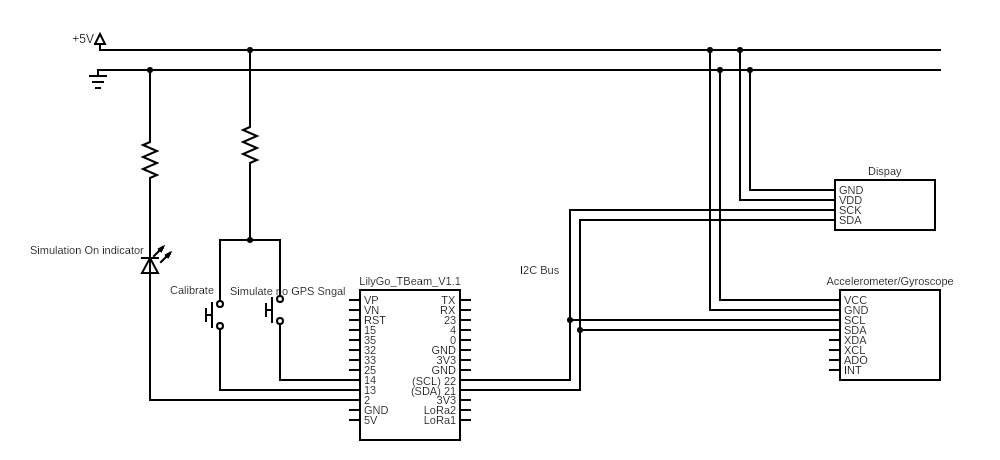
\includegraphics[width=15cm]{img/circuit.png}
    \caption{Circuit scheme (power supply of the TBeam board and power lines connection left out)}
\end{figure}
${}$

% SECTION 2: DATA PROCESSING
\section{Reading and processing accelerometer and gyroscope data}
The main challenge of the processing the accelerometer data is the fact that we receive the acceleration relatively to the accelerometer module and not relatively to the earth coordinate system and we need to convert them so we can calculate the final location. Furthermore, for the conversion we need an orientation of the board relatively to the earth coordinates which is not so easy to get without a tilt sensor or something similar.

\subsection{Processing and converting raw data}
As mentioned earlier, we obtain the accelerometer data relatively to the module axis. From the accelerometer and gyroscope we receive three 16-bit integers that correspond to the acceleration in x, y and z axes multiplied by 16384 in multiplies of $g$. After these 3 numbers, there follow three other 16-bit integers that correspond to the angular speed around x, y and z axes multiplied by 131 in degrees per second.\par
For this part, let's assume that we know the exact orientation of the module relatively to the earth coordinate system. If we know the orientation we can easily convert received acceleration data to the earth coordinates system that we convert received acceleration vector to the polar coordinates system, than we can easily rotate the vector by the orientation vector and then convert back to the Cartesian coordinates system and we obtain a vector of accelerations in x, y and z axe relatively to the earth coordinates system.

\subsection{Device calibration}
In this section I will talk about the way how can be obtained the orientation of the accelerometer module relatively to the earth coordinates system using only gyroscope and accelerometer. The calibration is a process that starts after a user presses the calibrate button and takes ca 10 seconds. During the calibration the device can be rotated as desired, but it must not move for the whole time. The main goal of the calibration is to obtain the orientation of the module relatively to the earth coordinates system. During the calibration we also calibrate the gyroscope so that it measures the correct data.\par
If the device is in calm, we expect the acceleration 0 in x and y axes and -1 $g$ in z axe\footnote{This is caused by gravity, the $[0,0,0]$ acceleration would be measured if the module was in a free fall} if the module coordinates would be the same as the earth coordinates. During the calibration time we measure the current acceleration. In order to minimize the error of the measurement, we measure the acceleration multiple times and after we have enough measurements we can calculate the average value and use it for the further calculation. After theses measurements we have information about the calm acceleration relatively to the module which is usually different from the expected $[0,0,-1]~g$ vector. At this point we can convert both vectors to the polar coordinates system and calculate the rotation differences between both vectors. In other words, we can calculate how we should rotate the measured vector so that we obtain the expected vector, which is the information about the module orientation that we need for the conversion to the earth coordinates system.\par
At this point we know the initial orientation of the device. But this orientation can change during the usage of the device and changes quite often. To handle this, we can use the data from the gyroscope. The gyroscope measures the angular speed of the module, so if we detect that there is some angular speed around any axe different from 0, we know that the user tilted the device, and we can accordingly adjust our information about the orientation. Updating the orientation is the only part for which I am using the gyroscope in the project.\par
The last thing I am doing during the calibration process is the calibration of the gyroscope. Because of the construction error, almost each gyroscope has shifted the 0 levels of the angular speeds. During the calibration process I can also measure the gyroscope values (and calculate their average). Because the device is in calm, the measured values should be all 0, but because of the shift error, each value is shifted, so we obtain the error shift values that we can further subtract from the measured values in order to get the right angular speeds. 

\subsection{Data smoothing}
From this point we know how to recalculate the measured values to the earth coordinates system, so we will assume that all accelerations are in the earth coordinates system.\par
In this section I will talk about the preparation of the measured data before we can start the final computation of the speed and location. The problem, why we shouldn't directly calculate speed and location from the measured date, is that because of the double integration, even small measurement errors can have huge consequences, and we have to minimize these errors as much as possible. If we observe the values from the accelerometer, we can see that they are "oscillating" around a real acceleration\footnote{This can be easily observed, if the device is in calm and the acceleration oscillates randomly around 0} (See figures 2 and 3). This phenomenon could be partially solved with smoothing.\par
Now we assume that we have measured some data, let's say $n$ records, and we want to smooth them. Let's choose a value $b$ and divide the set of measured records into $\tfrac{n}{b}$ blocks of $b$ consecutive records. In each block we will find a median value of each $x$, $y$ and $z$ axe and set all records in the block to this median. This will cause that we will avoid or smooth these oscillations or a noise in the form of several random completely wrong records.\par
This smoothing technique is really simple, fast and reduces the errors quite well. The disadvantage of the smoothing is that we partially lose the precision level of the measurement. For example, if there were some really short acceleration that took only a short time, it could be assumed as an error and completely ignored. Or if we have a block where the acceleration is changing, we would lose the information about the shape of the curve, how the acceleration is changing, and we would assume it later as linear.\par
The level how much the data will be smoothed and how large the information lost is depends on the value of $b$. If we chose very small $b$, in the extreme case $b = 1$, we wouldn't lose almost any information, but we would smooth really small blocks, so the smoothing wouldn't have almost any effect and most of the errors will remain. On the other hand, if we choose a really large $b$, in extreme the case $b = n$, we will ignore almost all errors, but also almost every information we obtain, so the data would become almost useless.\par
In this project, I chose $b = 16$ records\footnote{And I am working with data sets with $n=512$ records, so I divide them into 32 blocks. More about it in the next section.}. It is quite small, so we wouldn't lose almost any information, because the change of the acceleration is in reality not so fast that the curves inside each block can be almost every time quite good approximated to the linear values. But it is not too small, and it smooths data quite well, especially if the device is not accelerating at all.\par
\begin{figure}[h]
    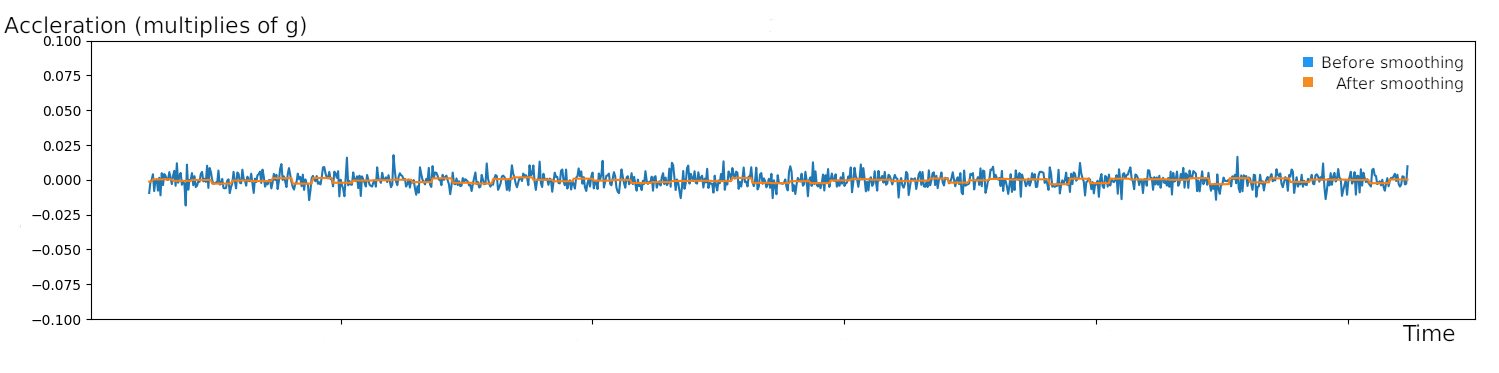
\includegraphics[width=15cm]{img/calmSmoothing.png}
    \caption{Acceleration on the x axe before and after smoothing when the device is in calm}
\end{figure}
\begin{figure}[h]
    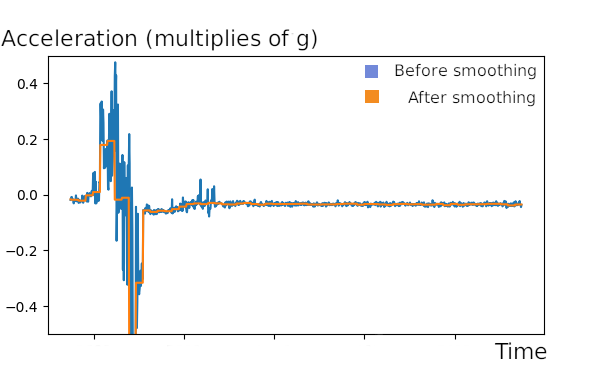
\includegraphics[width=15cm]{img/motionSmoothing.png}
    \caption{Acceleration on the x axe before and after smoothing when the device is in motion}
\end{figure}
After the data are smoothed, we could apply another technique to reduce an error. Even after smoothing, if the device does not accelerate, we can still get some small positive or negative accelerations, which need to be removed. To do that, we can choose some limit $l$ and then assume every acceleration, which is in the absolute value lower than the limit, as 0. For the project, I chose $l = 0.03125~g$.


\subsection{Calculating final speed and location}
Now we have reduced the measurement error, and we can finally calculate the final location. Let's assume we know the initial speed $v_0$ and location $p_0$ of the device\footnote{The initial speed will be 0 after calibration or result of the last calculation. The initial position will be last the record from GPS, before we lost the signal or result of the last calculation} and the set of $n$ last acceleration measurements together with the times of the measurement.\par
To calculate a velocity and a position from the acceleration, we need to convert the discrete values into a continuous function. Because the time differences between measurements are quite small, compared to expected accelerations, we can assume that between every 2 measurement results there is the acceleration constant and approximate our discrete function to the continuous one in the way displayed in the Figure 4.\par
\begin{figure}[h]
    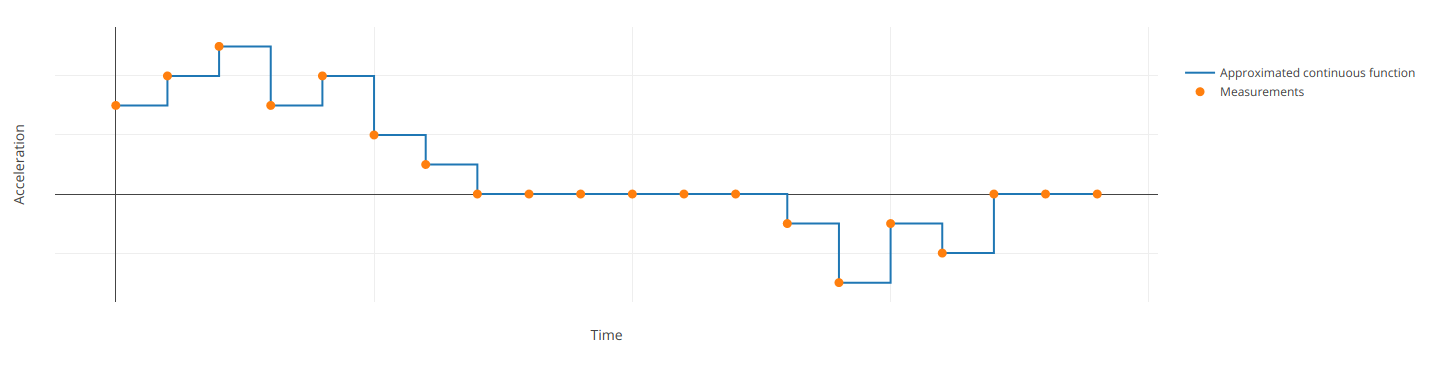
\includegraphics[width=15cm]{img/DiscToCont.png}
    \caption{Approximating discrete measurements to continuous function}
\end{figure}
Now, we have all information we need to calculate a velocity as
$$
    v(t) = v_0 + \int\limits_{T_\text{start}}^{t} a(\tau)~d\tau
$$
Where $v_0$ is initial speed, $T_\text{start}$ is a time of the first record in the measurements set, $T_\text{end}$ is time of the last record and $a(t)$ is the approximated acceleration function from the measurements. The value $v(T_\text{end})$ will be final speed used as initial speed for the next measurement.\par
When we know also the function of velocity with respect to time, we can integrate it again to obtain our relative position with respect to the last know position.
$$
    p_r = \int\limits_{T_\text{start}}^{T_\text{end}} v(t)~dt
$$
Now we have a relative position $p_r$, so we can convert it from meters to longitude and latitude degrees and add it to the last known location $p_0$ and obtain our current location.\par
The last thing we have to do is to choose the appropriate number of records $n$ that we will collect before we recalculate the location. If we chose $n$ relatively small, we would recalculate the position quite often, so the user would see the information about the position always up to date. If we chose $n$ quite large, it would take some time before we collected enough data to recalculate the location, and the user would have to wait some time before he/she sees the new updated values. But on the other hand, the larger $n$ we choose, the more data we have to calculate and we can perform more appropriate error correction, function approximation, and we also have denser data because we only collect them and we do not always recalculate the position, so we can obtain more accurate values.\par
In the project, I chose $n = 512$. We have quite enough data to do appropriate error corrections and collecting + recalculating takes a bit less than one second, so the data is almost always up to date\footnote{The target user is a human not another machine, so updating state in less than one second is fast enough}.

\subsection{Position recalculating pseudocode}
If I sum up all previous steps into a pseudocode, it will look like this.
\begin{enumerate}
    \item Let $v_0$ and $p_0$ be initial speed and location
    \item measure data until you have $n$ records
    \item smooth the data
    \item $v$ := calculate speed from the smoothed data
    \item $p$ := calculate relative position from the smoothed data
    \item $p'$ := convert relative position to the earth the coordinates units
    \item $p_0 := p_0 + p'$
    \item $v_0 := v$
    \item delete measured data
    \item goto step 2
\end{enumerate}


% SECTION 3: RESULTS
\section{Results and precision}
Now let's talk about the results and the precision I achieved with the accelerometer. To measure the precision, we can define an error as a ratio
$$
    E = \left|\frac{p_e - p}{p_e}\right|
$$
where $p_e$ is the expected relative position\footnote{Measured with my phone} and $p$ is the position calculated by the device.\par
For quite short distances, up to 10 m, the device was working quite well, with $E < 0.1$, which corresponds to the error lower than one meter for every 10 meters.

\begin{figure}[h]
    \centering
    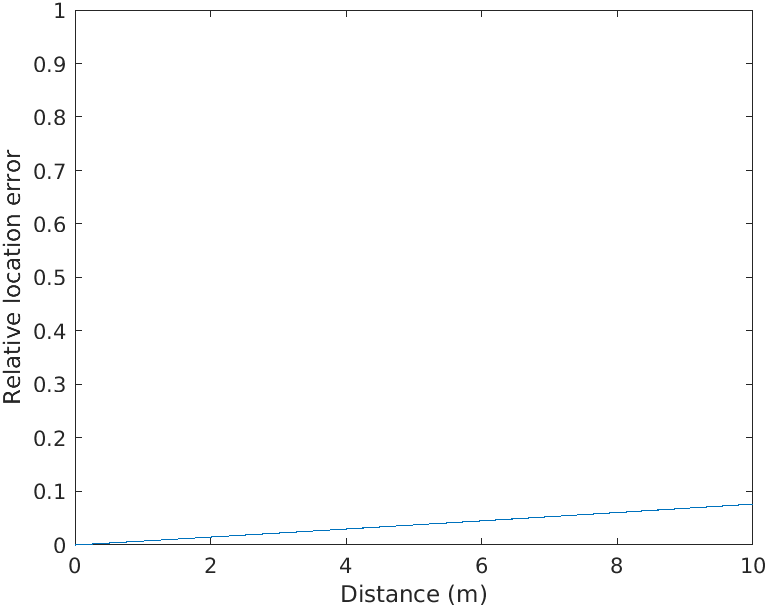
\includegraphics[width=8cm]{img/smallDistanceError.png}
    \caption{Device error for small distances (average from several measurements)}
\end{figure}

But if we continue with the measurement for the larger distances, from several tens to several hundred meters, we will see that the error grows exponentially and is quite soon really huge. If we recalibrate the device during the measurement and then continue measuring, we will shortly stop the grow, but after quite a short while we will get back to the exponential grow.\par
\begin{figure}[h]
  \begin{subfigure}{7.5cm}
    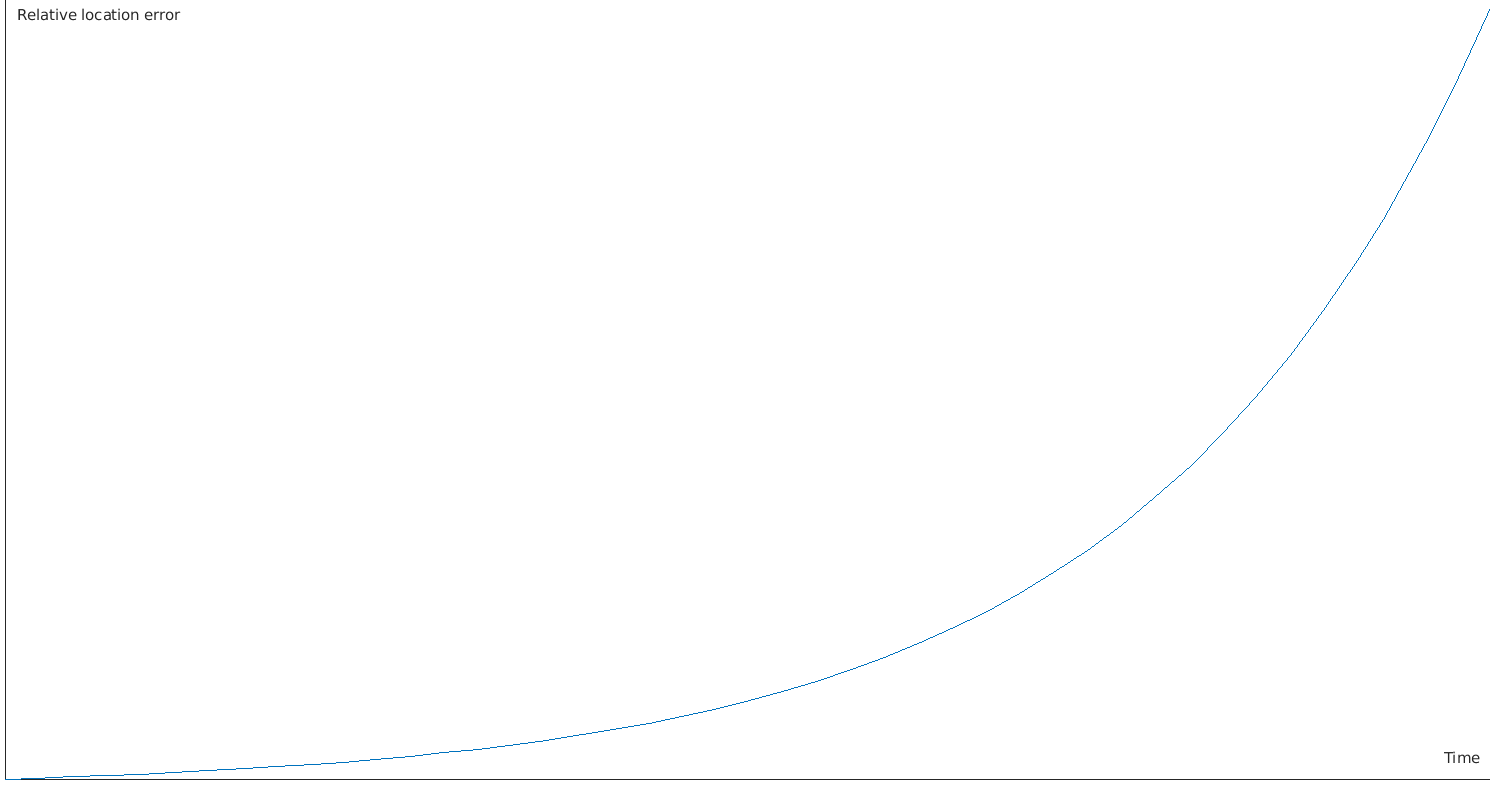
\includegraphics[width=7cm]{img/largeDistanceError.png}
    \caption{Without a calibration}
  \end{subfigure}
  \begin{subfigure}{7cm}
    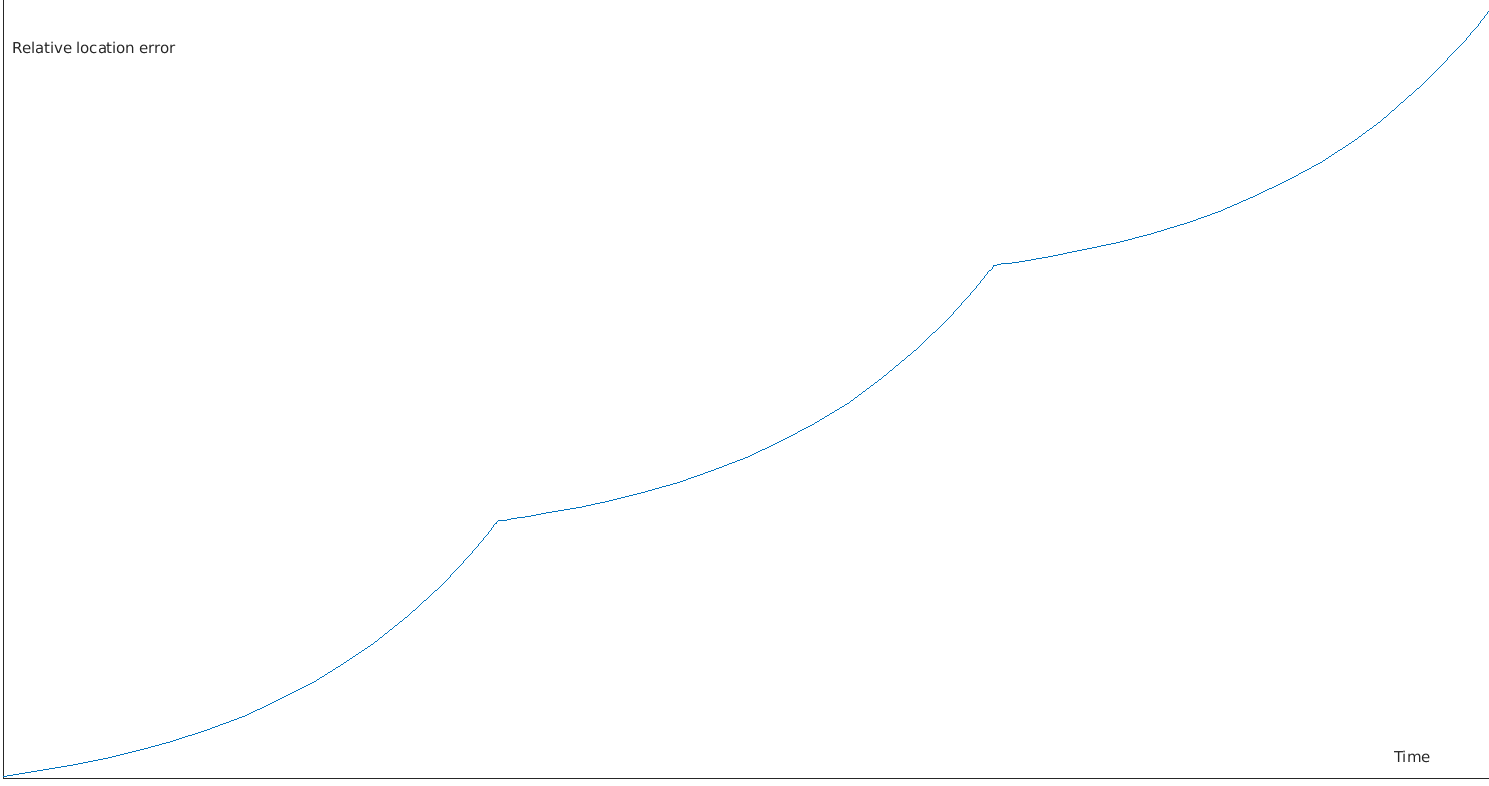
\includegraphics[width=7cm]{img/calibrationError.png}
    \caption{With 2 calibrations}
  \end{subfigure}
  \caption[Caption for LOF]{Device error tendency for larger distances\footnotemark}
\end{figure}

\footnotetext{I deliberately left out the units because the actual numbers were different for each measurement, depending on how much I was accelerating, changing directions or rotating with the device, but the tendency and shape of the curve was always the same.}
The question is, why is the error growing exponentially. One reason is the double integration of the acceleration, the error of the acceleration measurement will be propagated\cite{UNCERNITY} and ends up in the exponential of its value, so it has large consequences even if it is quite small. The other reason is that the value depends on the previous results, especially on the previous velocity, and if these values are wrong because of the measurement error, the next error would be larger and larger, which also leads to the exponential grow of the error.\par
But the main factor causing the error is the translation from the accelerometer coordinate system, in which the accelerations are measured, to the earth coordinates system. This translation depends on the knowledge of the orientation of the device, which is determined during the calibration and updated according to the data from the gyroscope, which can also be inaccurate, so after some time, we have a wrong orientation vector, which significantly increase the error of the data from the accelerometer (mainly because of the gravity vector which will be reflected also in $x$ and $y$ axes) which will lead to huge errors described in previous paragraph. The fact that the error stopped growing for a while after a recalibration also suggests that the main cause of the error is the wrong orientation.

% SECTION 4: CONCLUSION
\section{Conclusion}
In conclusion of this project, I would say that accelerometer is not an appropriate substitution for GPS and because of the errors described in the previous section, it is an inappropriate type of sensor for each application where we have to know a precise location in a different coordinate system, than the one which is relative to the sensor/device. Maybe if we would combine the accelerometer with a tilt sensor or any other sensor which allows direct measuring of the orientation of the device with respect to the earth coordinates system, then it could deliver better results, but the error of using only an accelerometer with a gyroscope is too large for any real application.\par

\clearpage
\pagenumbering{gobble}
\nocite{ACCGyro}
\nocite{BoardGH}
\nocite{NMEA}
\nocite{GYRO}
\printbibliography

\end{document}
